%% IMPORTANT! COMPILE WITH -shell-escape option for ffcode to work

\documentclass[a4paper,11pt]{article}
% Useful packages
\usepackage{amsmath}
\usepackage{amssymb}
\usepackage[utf8]{inputenc}
\usepackage[pdftex]{graphicx}
\usepackage{etoolbox}
\usepackage[svgnames]{xcolor}
\usepackage{tcolorbox}
\usepackage{fancyhdr}
\usepackage{matlab-prettifier}
\usepackage{enumerate}
\usepackage[shortlabels]{enumitem}
\usepackage{amsthm}
\usepackage{ffcode}

% Page size
\textwidth=170mm
\oddsidemargin=0mm
\evensidemargin=\oddsidemargin
\textheight=230mm
\topmargin=-10mm
%Section numbering
\setcounter{secnumdepth}{-1}
%opening
\title{EITF75: Lab 1A&B Report}
\author{Ola Davidsson and Emil Lantz}
\begin{document}
\raggedright
\maketitle
\section{Preparation exercises}
\subsection{Problem 1}
\subsubsection{a}

We know that F is 4 times smaller than Fs and we then calculate the equation below. 
\[
\omega_{0} = 2 \pi \frac{F_{0}}{F_{s}} 
\]
Resulting in
\[
\omega_{0} = \frac{\pi}{2}
\]
We also know that the zeroes comes in pair which mean we also have one at 
\[
\omega_{0} = -\frac{\pi}{2}.
\]
This means we have our zeroes along the y-axis and they can be written as
\[
(1-e^{j\frac{\pi}{2}}z^{-1})(1-e^{-j\frac{\pi}{2}}z^{-1})
\]
This gives us
\[
H_{1}(z) = \frac{(z-e^{j\frac{\pi}{2}})(z-e^{-j\frac{\pi}{2}})}{z^2} = \frac{z^2-2zCos(\frac{\pi}{2})+e^{j(\frac{\pi}{2}-\frac{\pi}{2})}}{z^2} = \frac{z^2+1}{z^2}.
\]
The last thing needed is to substitute 
\[
z = e^{j2\pi f} 
\]
Inserting this with f = 1/2 should give us 
\[
H_{1}(f) = 1 =  b_0\frac{e^{j\pi}^2 + 1}{e^{j\pi}^2} = 2b_0 \xrightarrow{} b_0 = \frac{1}{2}
\]
\subsubsection{b}
\begin{figure}[H]
    \hspace{-2.5cm}\includegraphics[scale = 0.3]{./images/pz-p1.jpg}
    \caption{Pole-zero plot}
\end{figure}
\subsubsection{c}
\begin{figure}[H]
    \hspace{-40pt}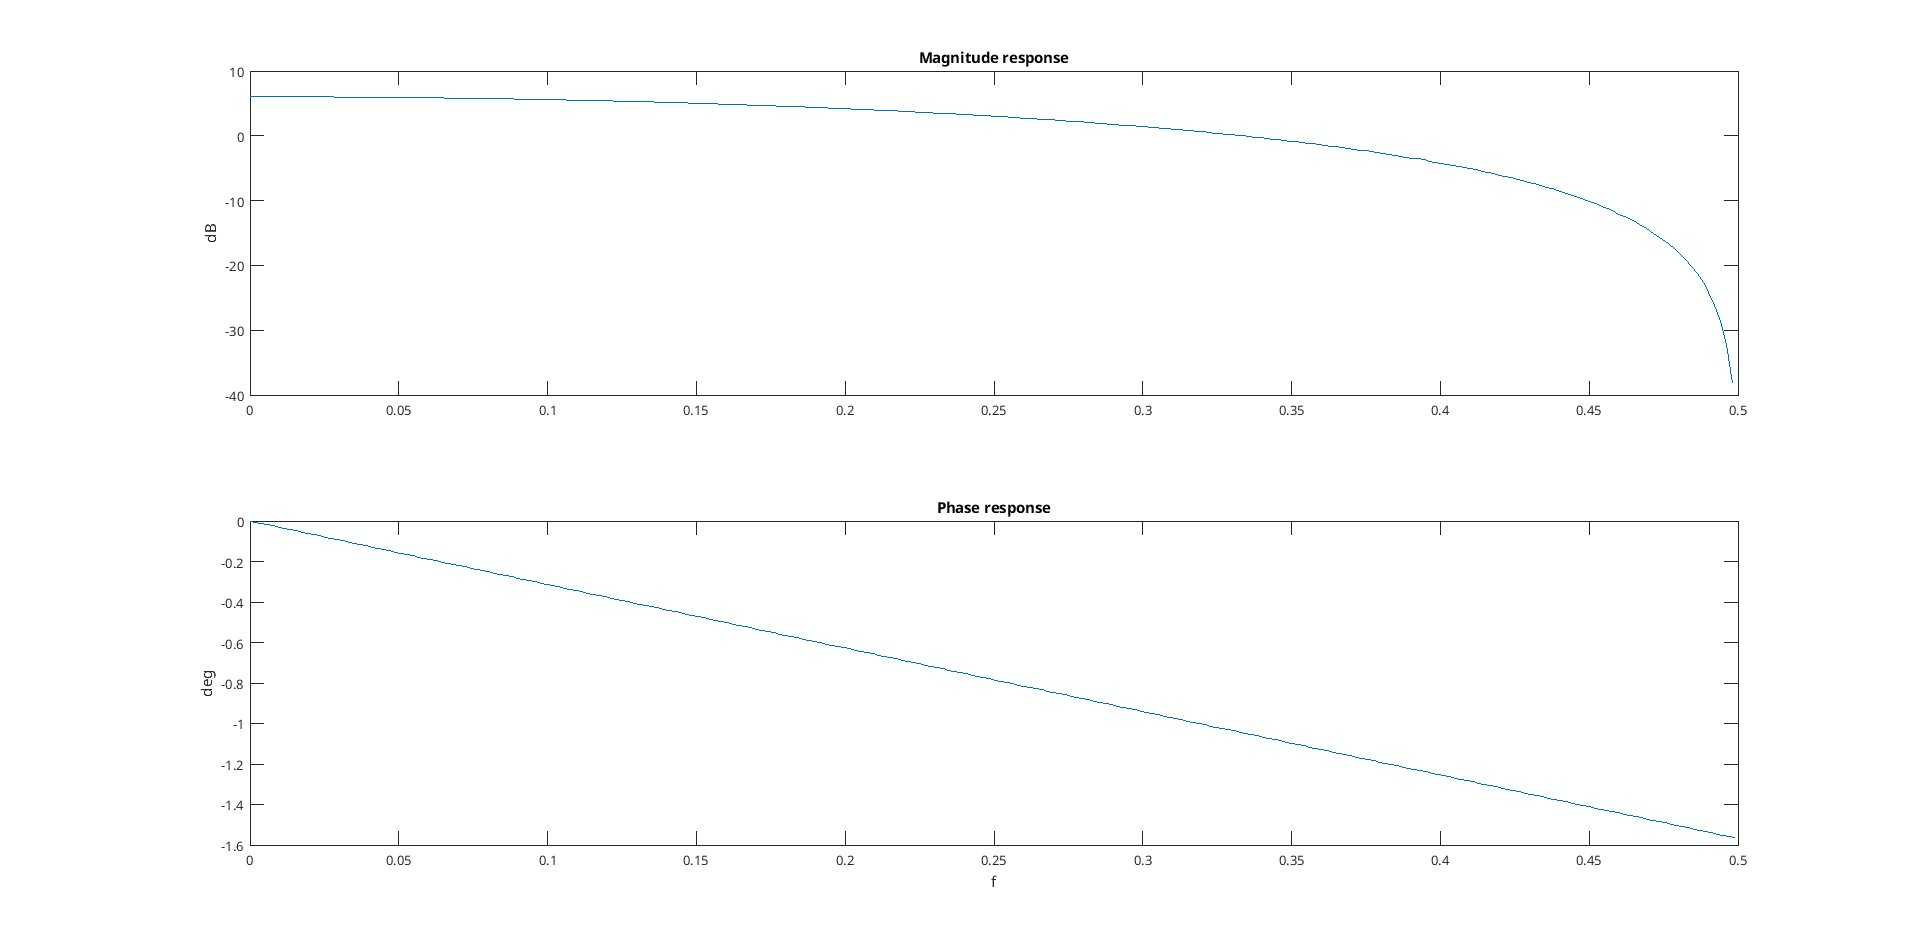
\includegraphics[scale=0.28]{./images/prep-1c.jpg}
    \caption{Magnitude and phase response plot for preparation exercise 1c}
    \label{fig:my_label}
\end{figure}

\subsection{Problem 2}
\subsubsection{a}
\[
H_{2}(f) = 1 =  b_0\frac{e^{j\pi}^2 + 1}{e^{j\pi}^2 + 0.95^2} \xrightarrow{} b_0 = 0.95125
\]
\subsubsection{b}
\begin{figure}[H]
    \centering
    \hspace{-60pt}\includegraphics[scale = 0.6]{./images/p2-pz.jpg}
    \caption{Pole-zero plot}
\end{figure}
\subsubsection{c}
\begin{figure}[H]
    \hspace{-40pt}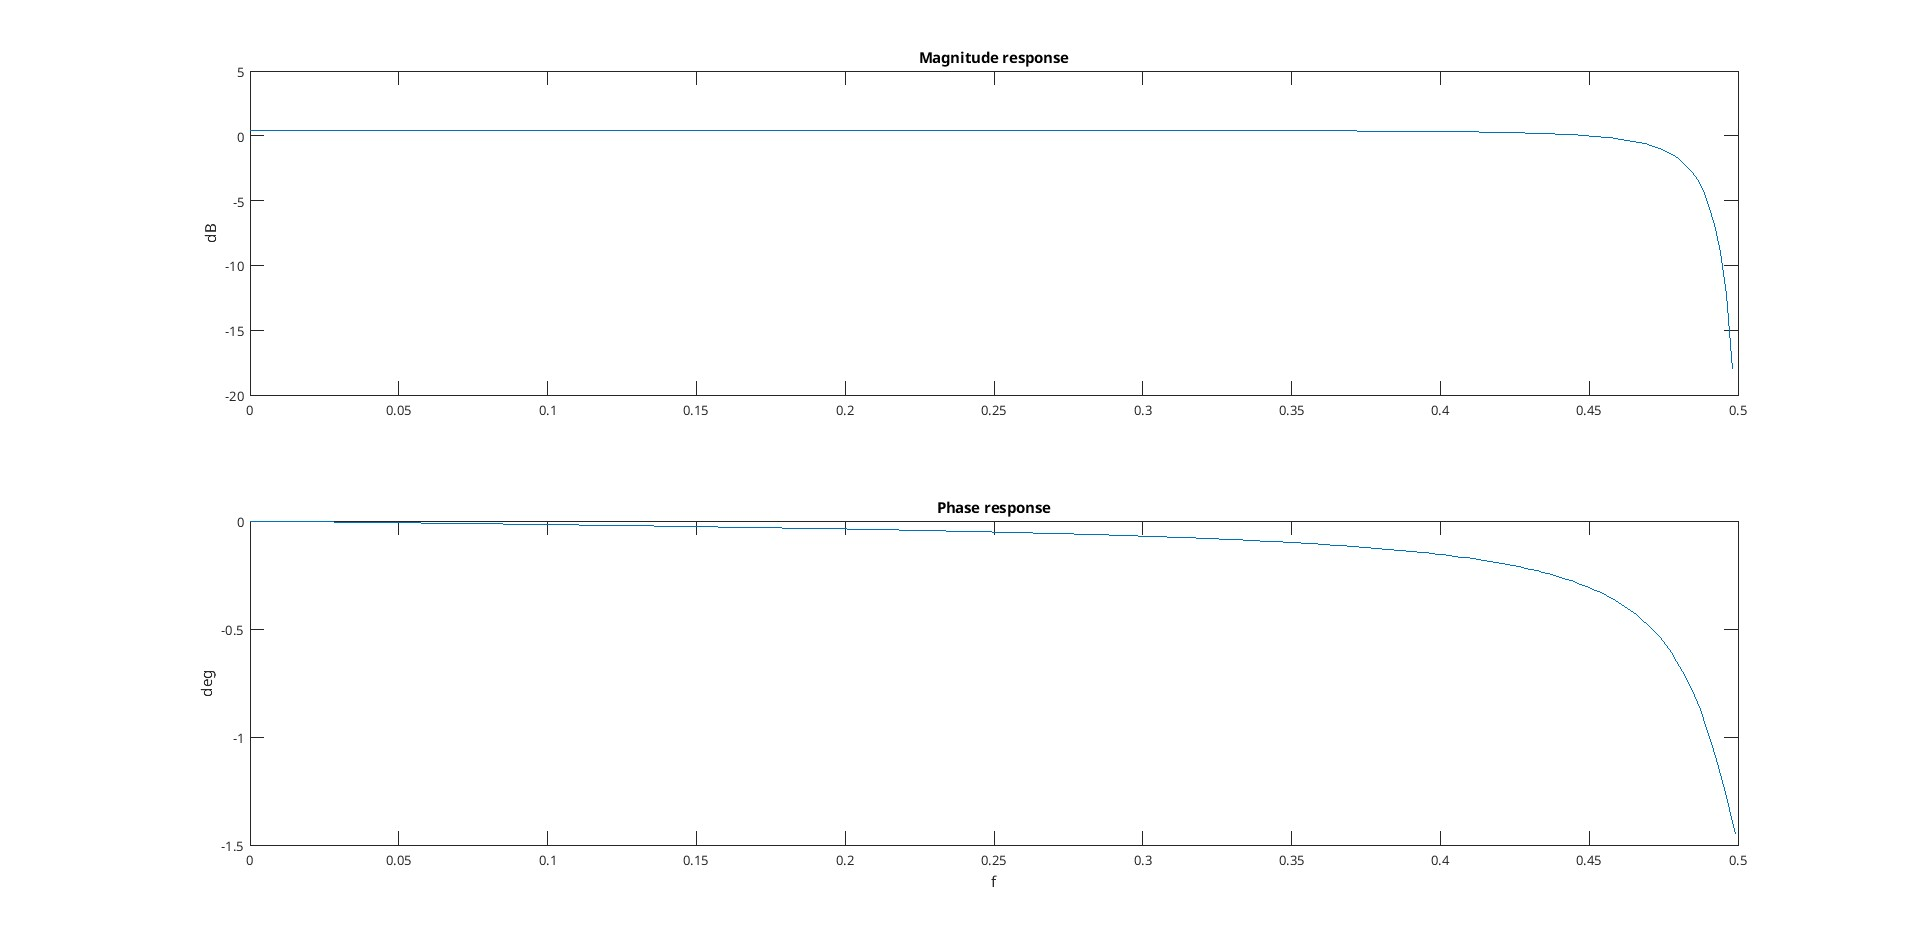
\includegraphics[scale=0.28]{./images/prep-2c.jpg}
    \caption{Magnitude and phase response plot for preparation exercise 2c}
\end{figure}
Our filter is now more accurate on the frequency that we want to remove. Before we have a dampening effect on more than the area we want to dampen. 
%Kolla skillnaden i fas graferna också. 

\subsection{Problem 3}
\subsubsection{a}
\[
y(n) = x(n) + \alpha x(n-D)
\]
Which gives us
\[
h(n) = \delta(n) + \alpha\delta(n-D)
\]
\subsubsection{b}
\[
H(\omega) = 1 + \alpha e^{-jwD}
\]
\begin{figure}[H]
    \hspace{-40pt}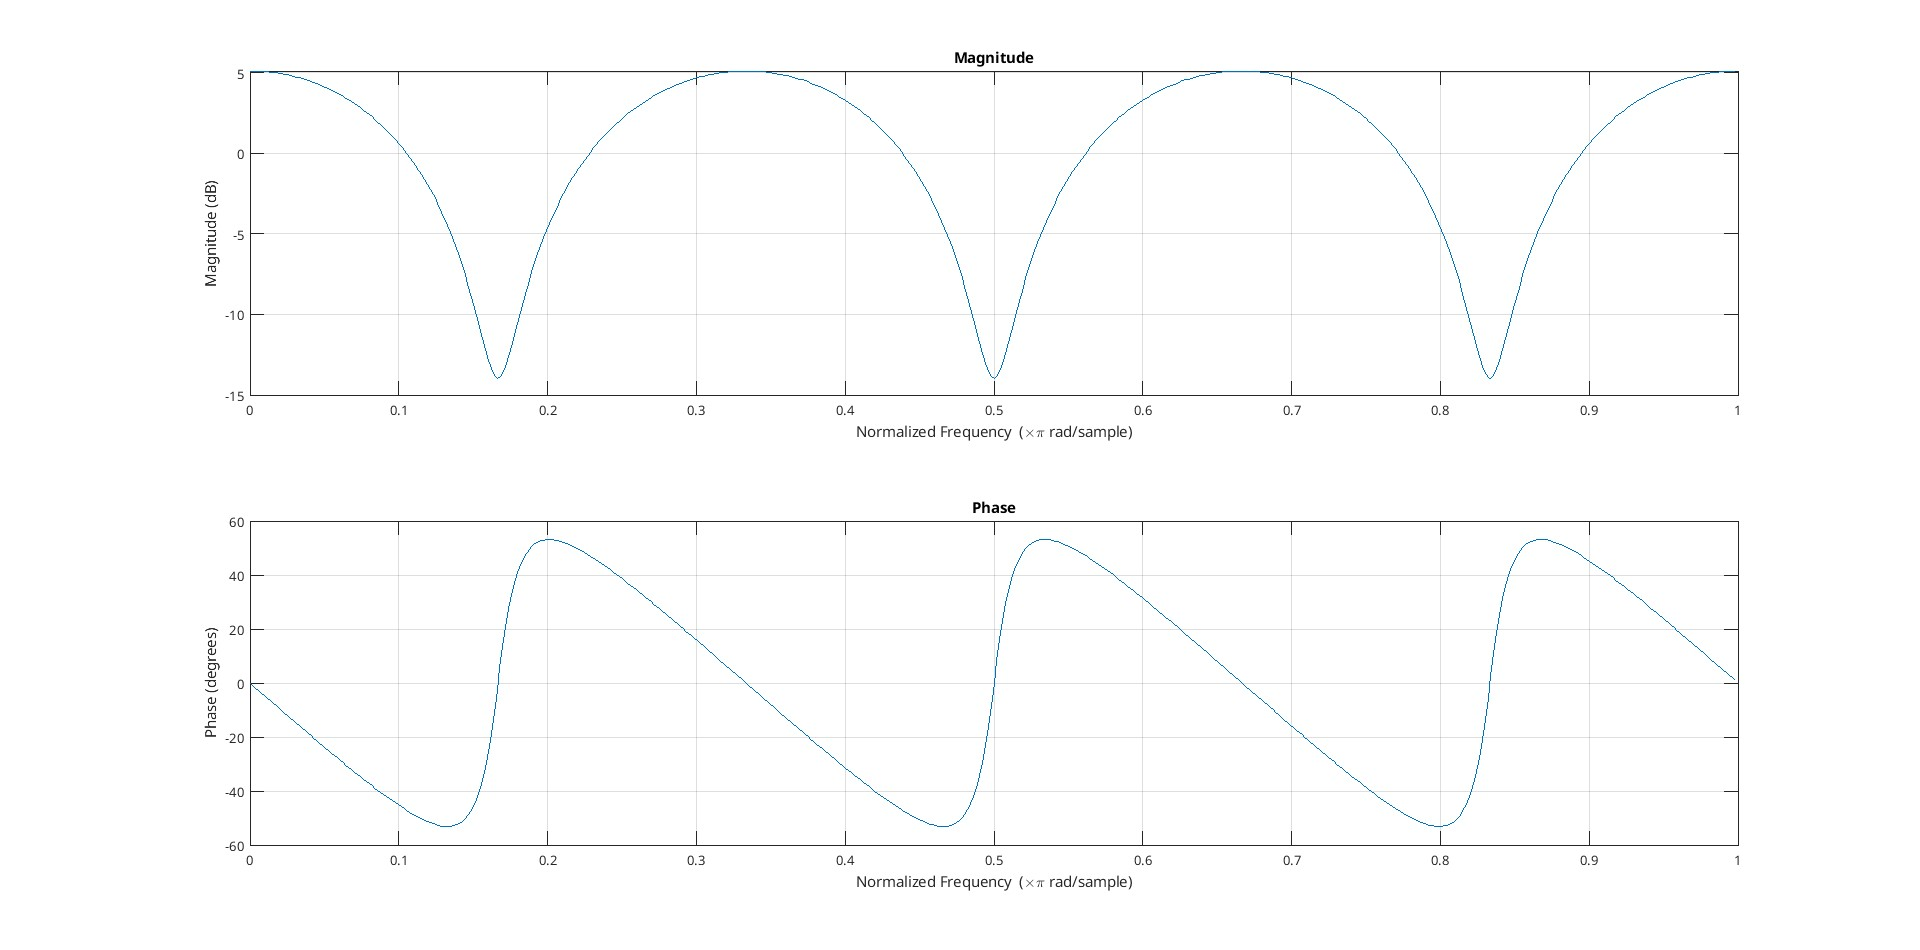
\includegraphics[scale=0.28]{./images/prep-3b.jpg}
    \caption{Plot of magnitude response asked for in 3b}
    \label{fig:my_label}
\end{figure}
\subsubsection{c}
\[
H(\omega)^{-1} = \frac{1}{1 + \alpha e^{-jwD}}
\]
Now going to the Z-transform of this we get.
\[
\frac{z^D}{z^D + \alpha}
\]
Which means we get D zeroes at Z = 0. And the poles at
\[
poles = \sqrt[D]{-\alpha}
\]
\subsubsection{d}
\[
H(\omega)^{-1} = \frac{1}{1 + 0.8 e^{-5jw}}
\]
\begin{figure}[H]
    \hspace{-45pt}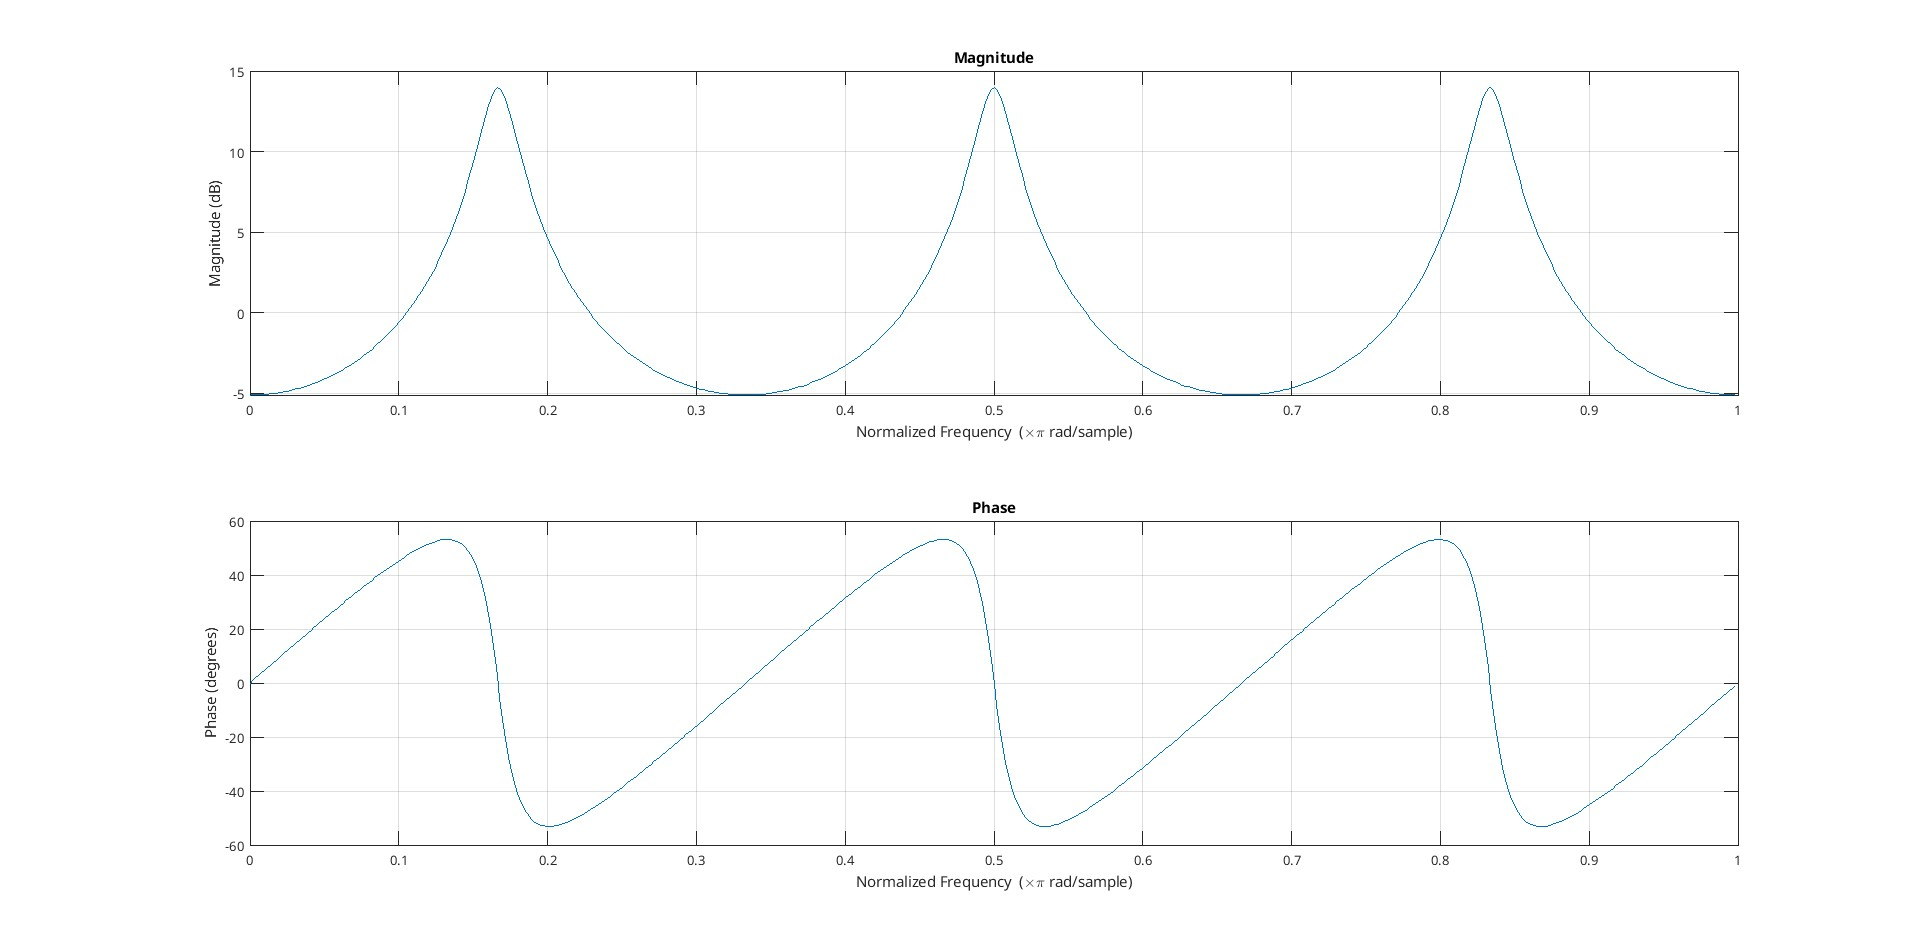
\includegraphics[scale=0.28]{./images/prep-3d.jpg}
    \caption{Caption}
    \label{fig:my_label}
\end{figure}
\subsubsection{e}
As long as 
$
|\alpha| < 1
$

\section{Laboratory tasks}

\subsection{Lab Task 1}
To playback the audio files as instructed in lab task 1, we used the following MATLAB code:
%This environment shows how to get 'nice' presentation of MATLAB code in LaTex:
\begin{ffcode} 
%% Task 1
%Read HQmusic.wav from file (y = signal, f = sampling freq.)
[y, f] = audioread('MATLAB_FILES/HQmusic.wav');
%Playback HQmusic.wav at reconstruction freq. f_pb (Change f_pb according
%to task)
f_pb = f / 2;
soundsc(y, f);
\end{ffcode}

It was noted that changing the reconstruction frequency ("f\_pb" in code) to half of the sampling frequency ($\frac{F_s}{2}$) both lowered the volume and made the pitch sound lower. Changing f\_pb to $2F_s$ had the opposite effect on the pitch.
\subsection{Lab Task 2}
The signal yielded from task 1 was plotted, both in the time and frequency domain. Time domain signal can be seen in figure 7 and the frequency domain signal can be seen in figure 8.

\begin{ffcode} 
%% Task 2
%plot time domain signal
secs = length(y) / f;
time = linspace(0, secs, length(y));
plot(time, y)
hold on
%plot freq. domain signal
Spectrum_PLOT(y, f);
\end{ffcode}

\begin{figure}[H]
    \centering
    \hspace{-40pt}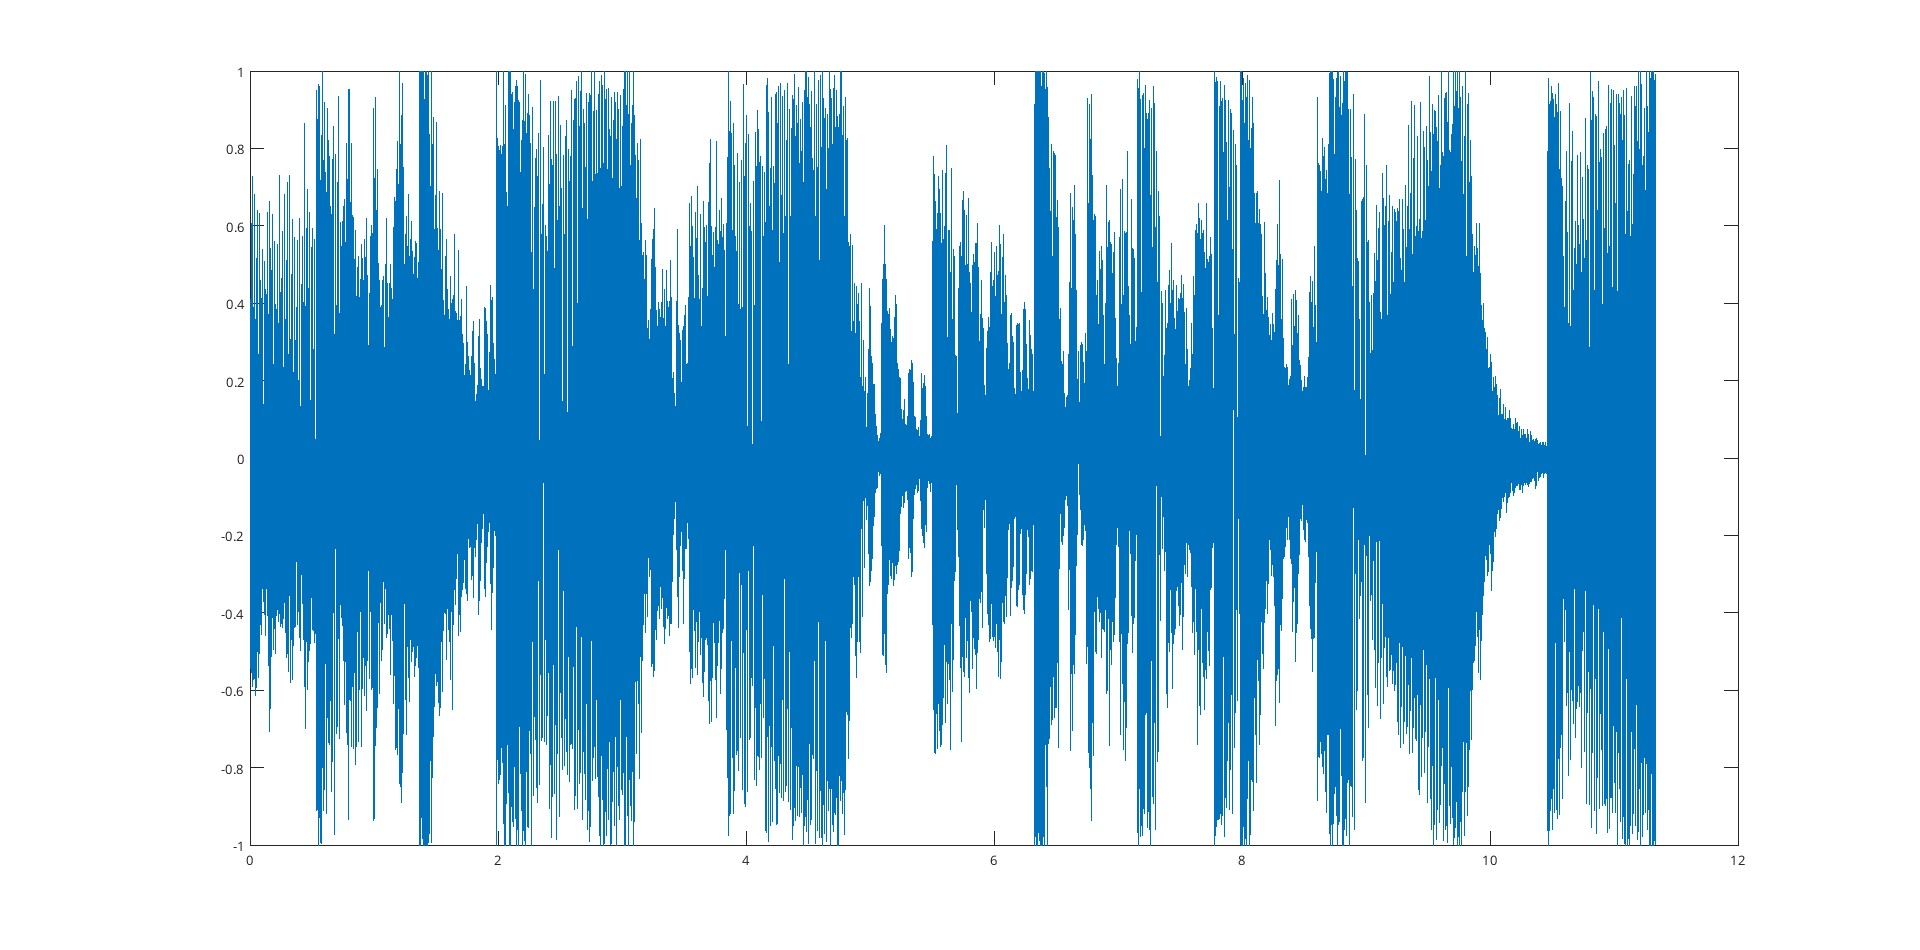
\includegraphics[scale = 0.2]{./images/Task2-PSD.jpg}
    \caption{Time domain plot of HQmusic.wav's signal}
    \label{fig:Task 2 Time domain}
\end{figure}

\begin{figure}[H]
    \centering
    \hspace{-60pt}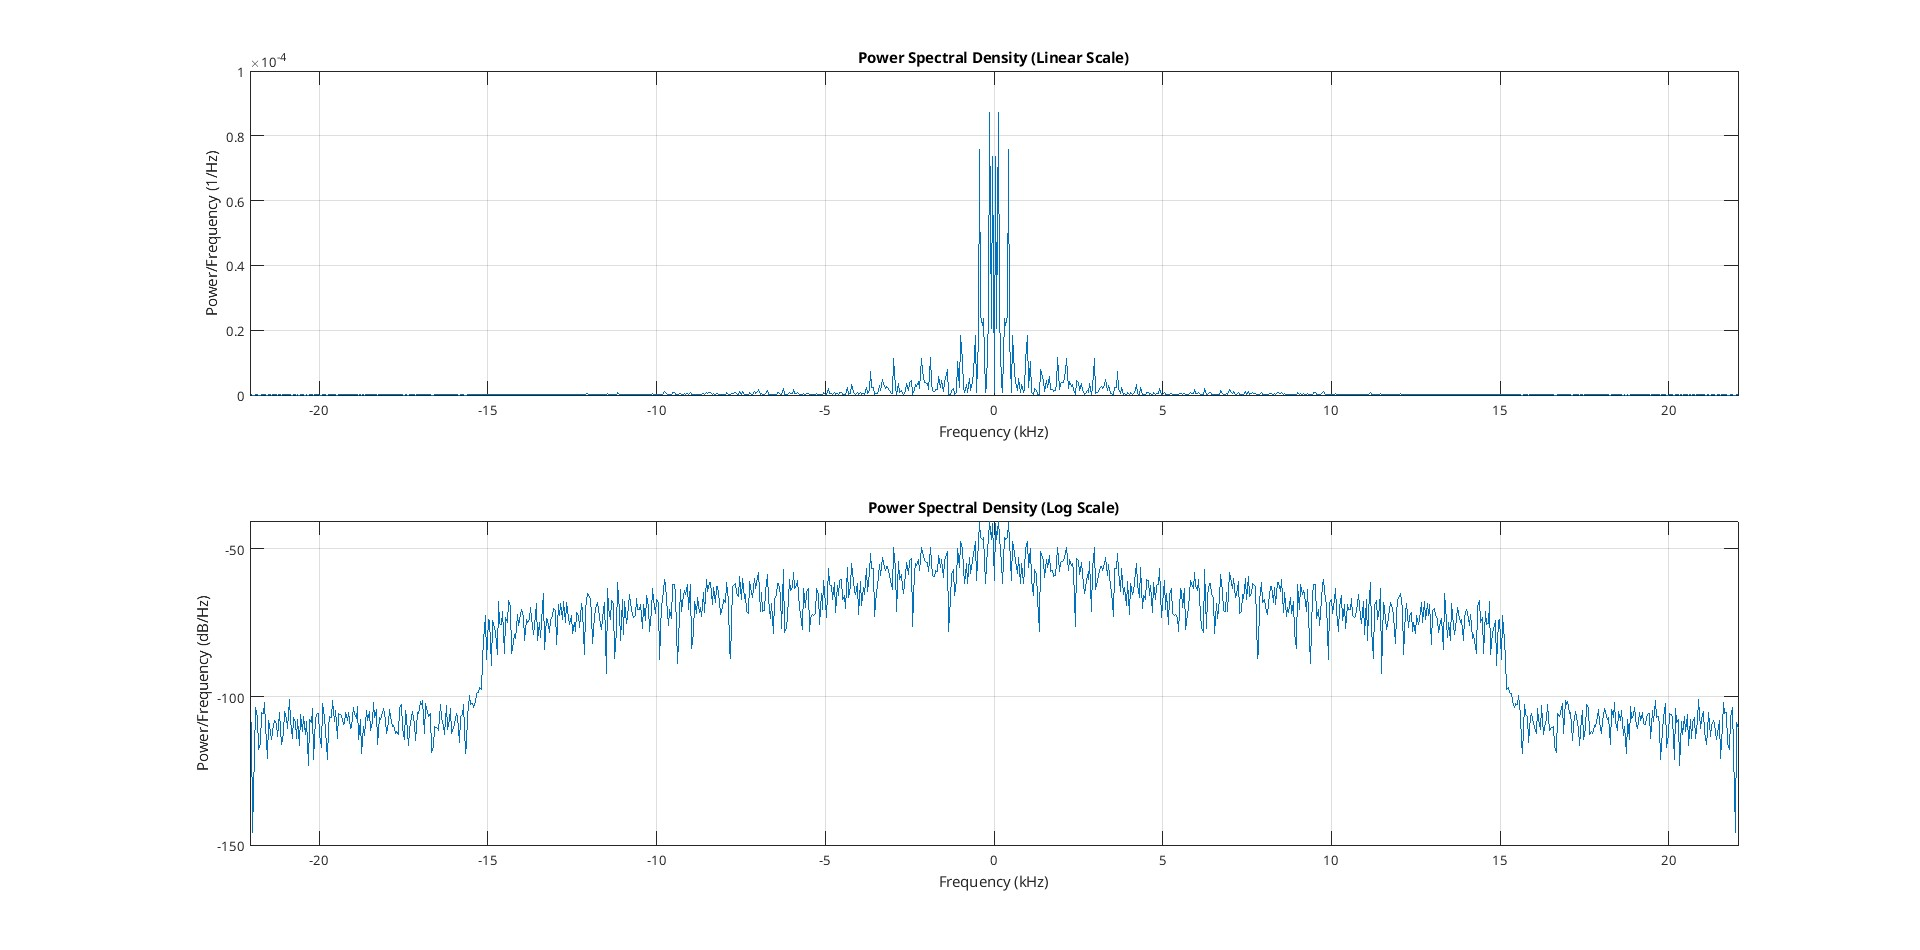
\includegraphics[scale = 0.28]{./images/Task2-FFT.jpg}
    \caption{Frequency domain plot of HQmusic.wav's signal}
    \label{fig:Task 2 Freq. domain}
\end{figure}


As can be seen in figure 8, the most prominent (largest) frequency component was 120 Hz. Since the audio was bass-heavy music, this is a reasonable result.

\subsection{Lab Task 3}
For task 3, a simple moving-average filter was applied to HQmusic.wav's signal. The following MATLAB code was used to apply the filter:

\begin{ffcode}
%% Task 3
filter = 1/5*ones(5,1);
%discard first 4 samples of output
u = conv(y, filter);
u = u(5:end);
soundsc(u, f)
Spectrum_PLOT(u, f)
\end{ffcode}

The filtered signal can be seen in figure 9.
\begin{figure}[H]
    \centering
    \hspace{-60pt}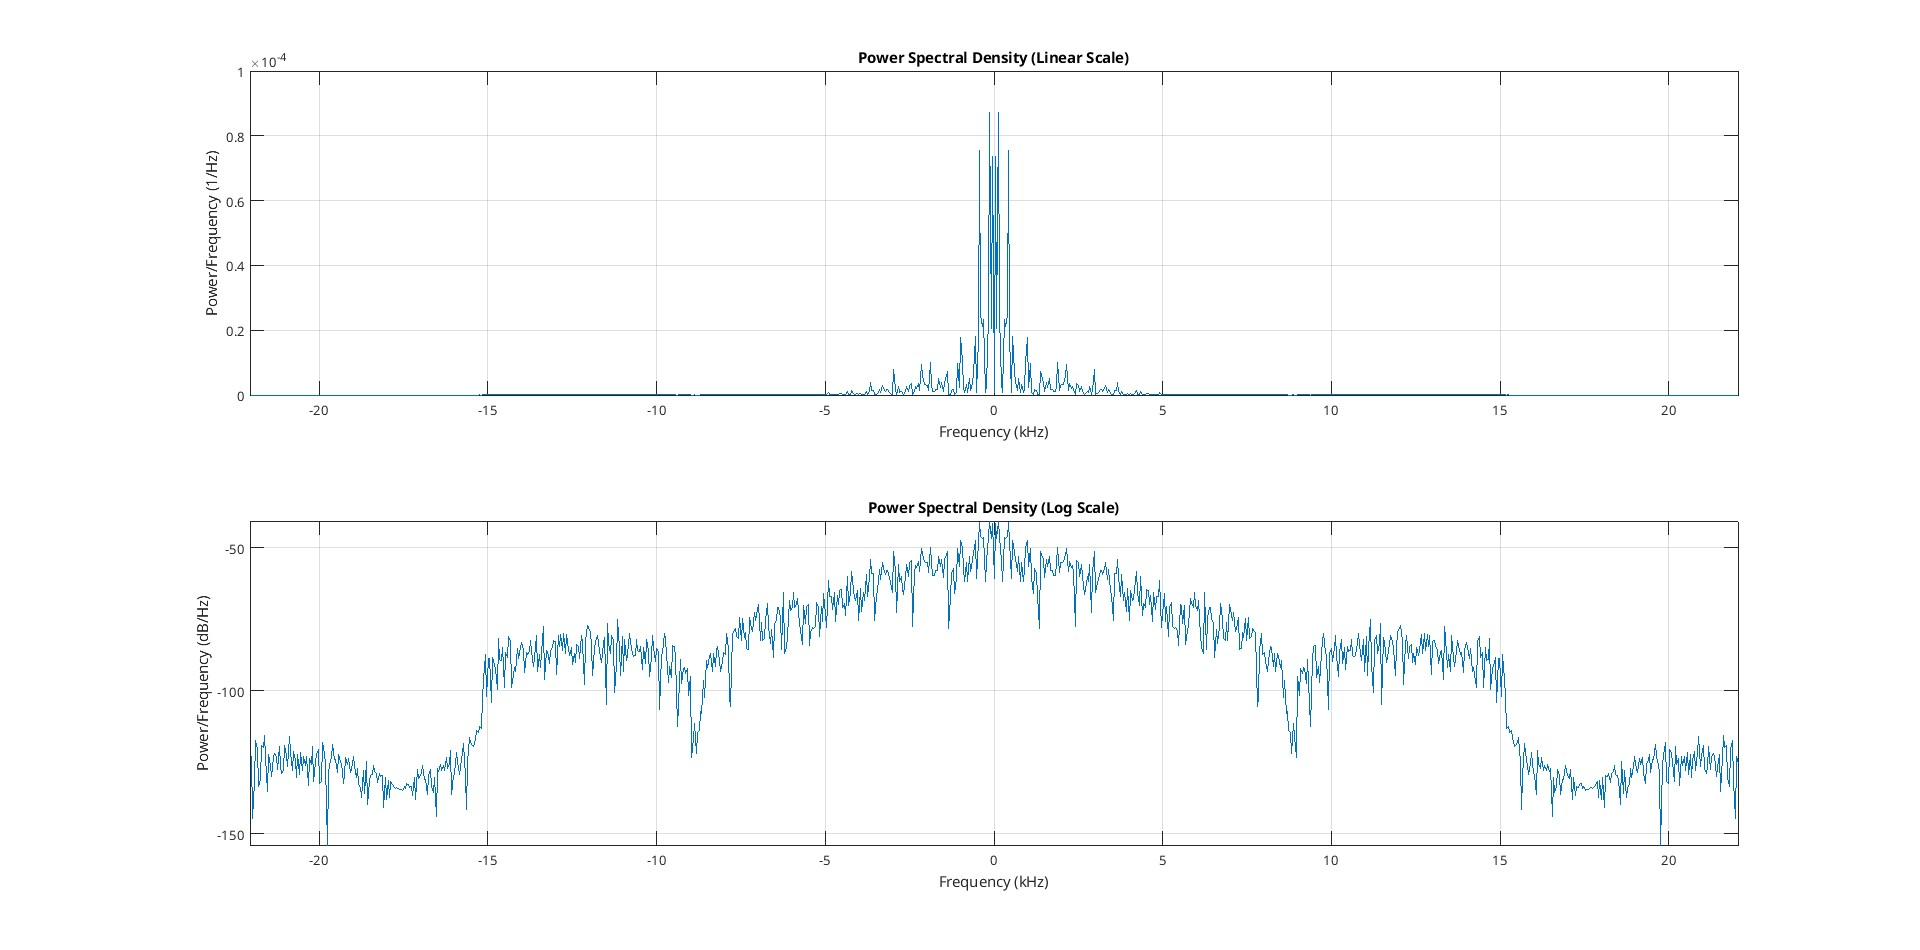
\includegraphics[scale = 0.28]{./images/Task3-filtered.jpg}
    \caption{Frequency domain plot of HQmusic.wav's signal, with a moving average filter applied}
    \label{fig:my_label}
\end{figure}
This filter removed more of the signals higher frequencies (treble). This is due to the filter taking the average amplitude of frequencies over 5 samples. Since higher frequencies are less prominent in the audio (as seen in figure 8), these frequencies are filtered. Increasing the length from 5 to 15 amplified this effect. Removing even more of the higher signals, leaving mostly bass.

Differences between the linear plots before and after the filter are minimal. The log-plotted figures, however, have notable dips around 8.9 kHz. The valleys starting at 15 kHz have a more rounded appearance after the filter.
\subsection{Lab Task 4}
For task 4 white noise was added using 
\begin{ffcode}
%% Task 4
% add noise
y_noisy = y + 0.1*randn(length(y), 1);
%soundsc(y_noisy, f)
Spectrum_PLOT(y_noisy, f)
\end{ffcode}
in MATLAB. The signal with added noise can be seen in figure 10.
\begin{figure}[H]
    \hspace{-55pt}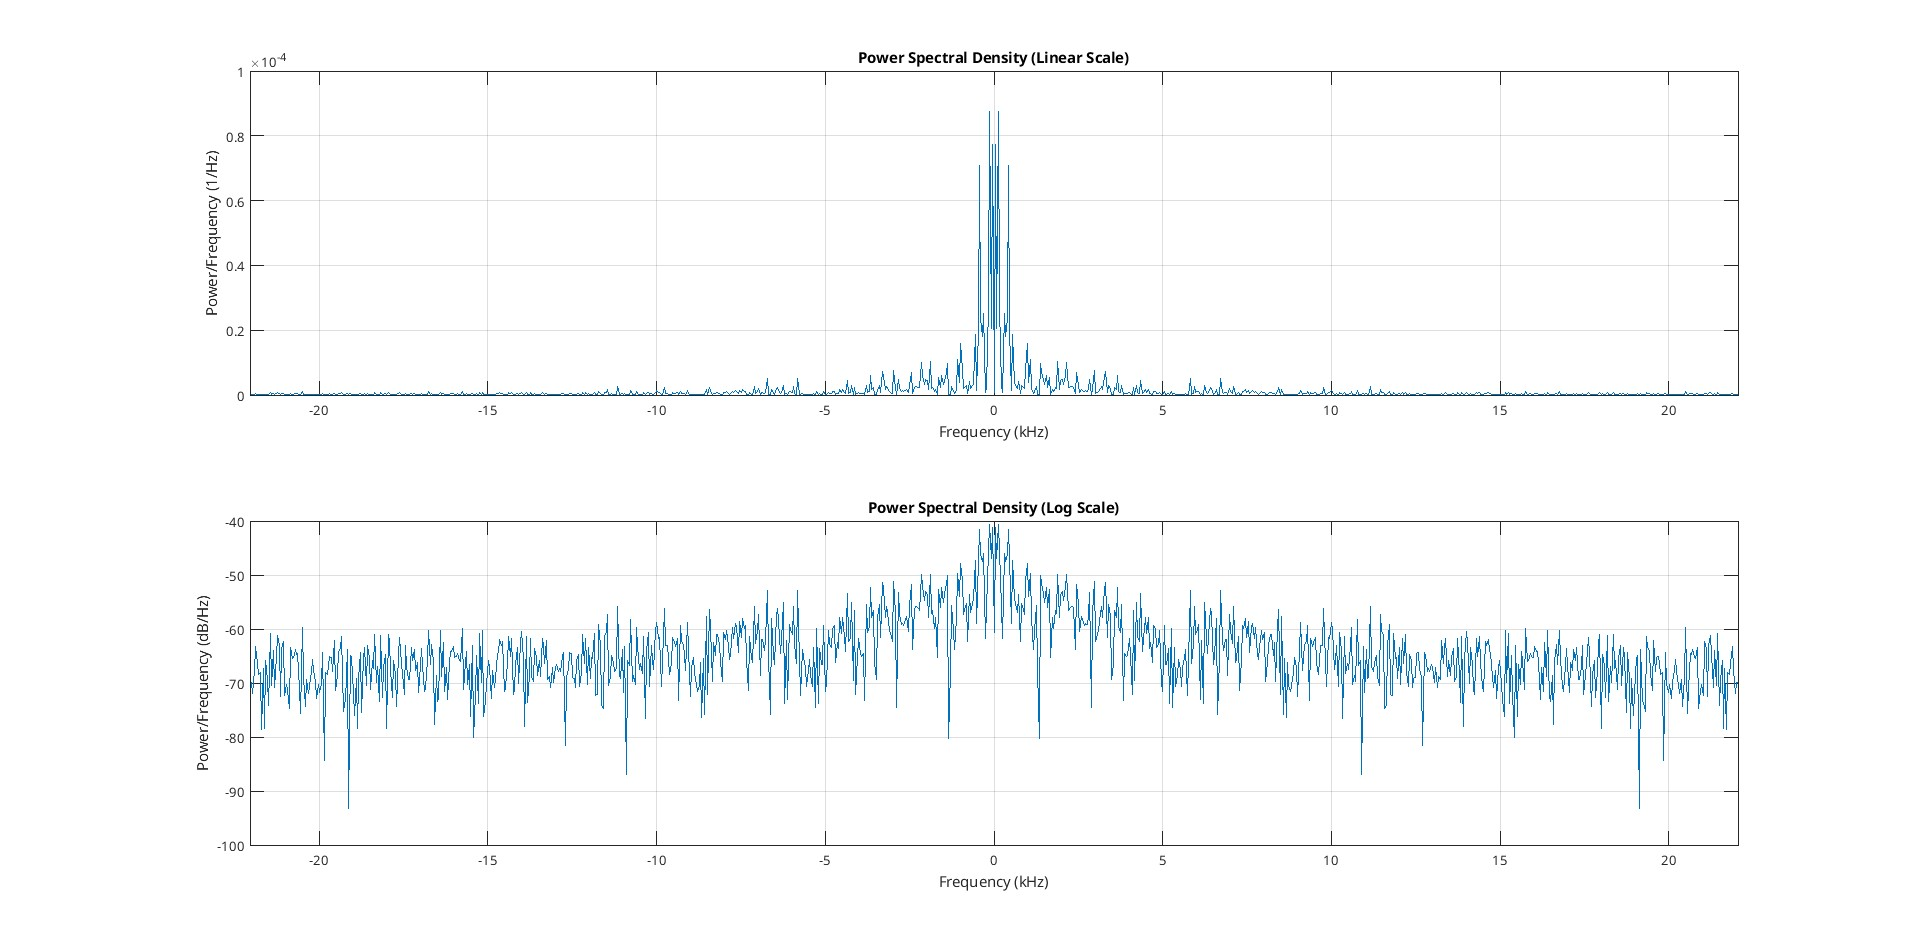
\includegraphics[scale=0.28]{./images/Task4-noisy.jpg}
    \caption{HQmusic.wav's signal with an added Gaussian white noise}
    \label{fig:my_label}
\end{figure}

Afterwards, the noise was filtered by passing the noisy signal through a moving average filter.
\begin{ffcode}
% filter noise
filter = 1/5 * ones(5,1);
u_noisy = conv(y_noisy, filter);
u_noisy = u_noisy(5:end);
soundsc(u_noisy, f)
Spectrum_PLOT(u_noisy, f)
\end{ffcode}
The plot of the filtered signal can be seen in figure 11.
\begin{figure}[H]
    \hspace{-40pt}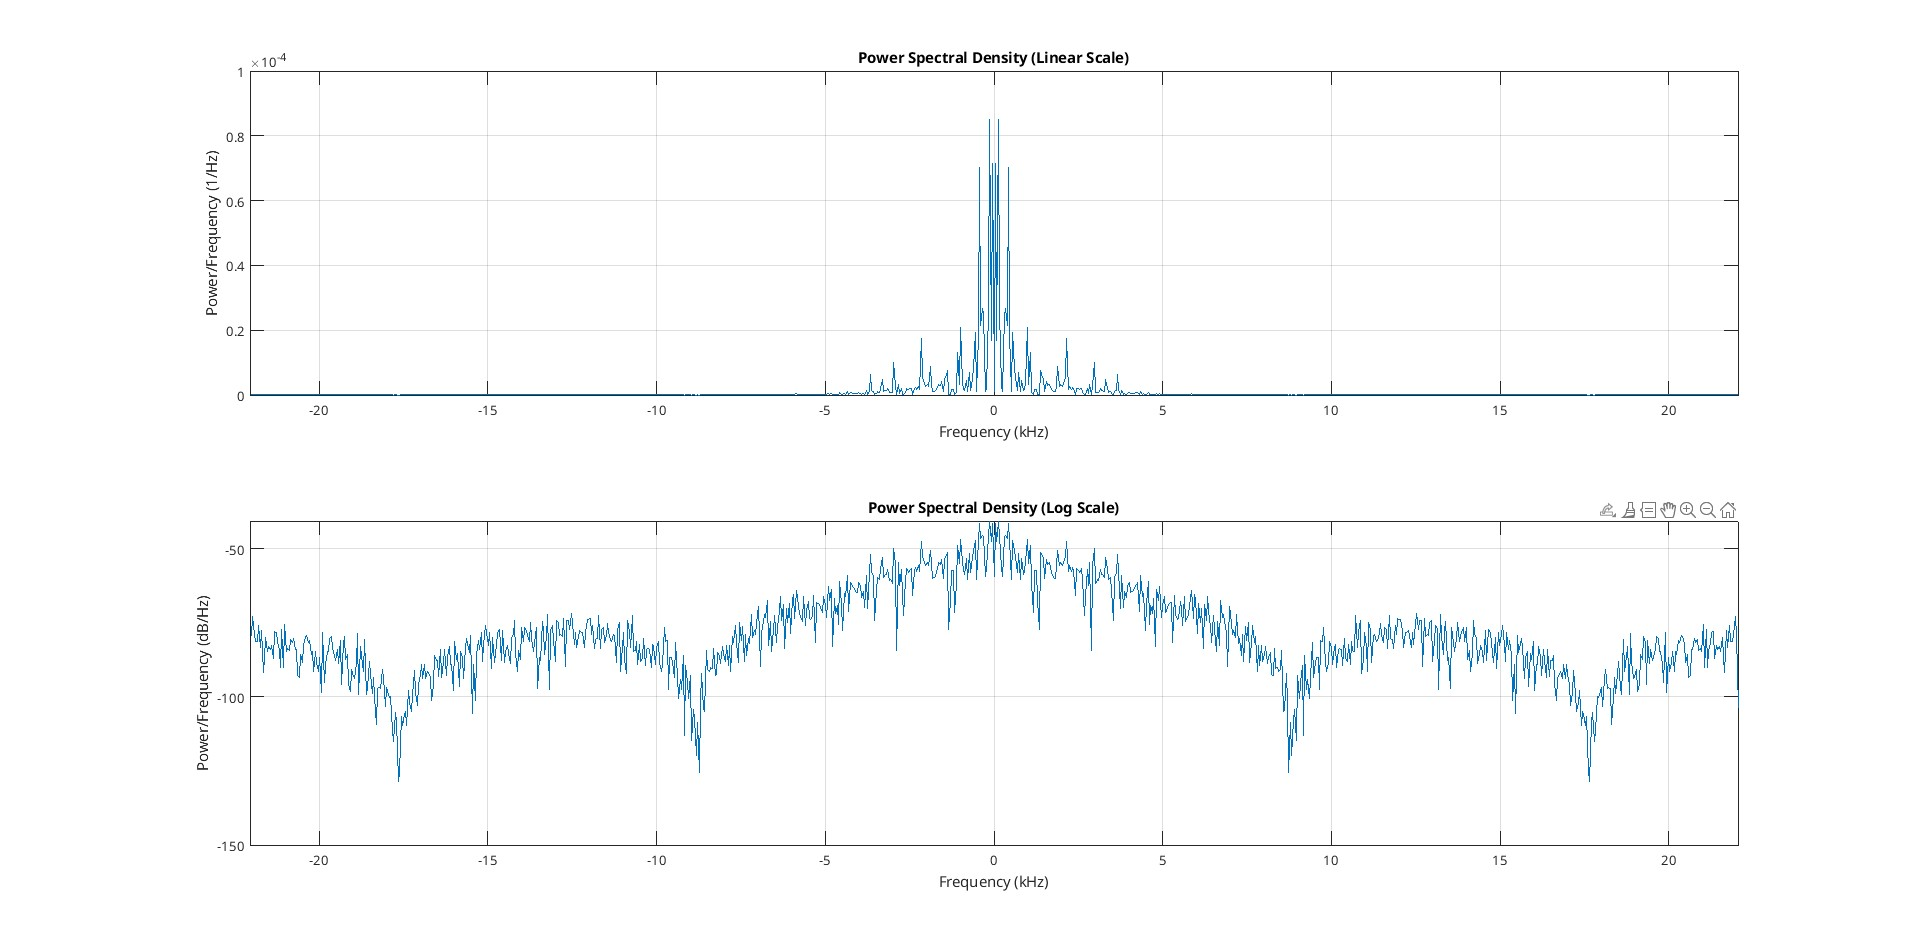
\includegraphics[scale=0.28]{./images/Task4-filtered}
    \caption{Signal from figure 10, passed through a moving average filter of length 5}
    \label{fig:my_label}
\end{figure}
% Nollställen i n*fs / 5 pga faltning med 1/5
As can be seen, the filter reduced the amplitude of the noise considerably (though it did not completely remove the noise), however some sharp dips can be seen around multiples of $\frac{1}{5} \cdot F_s$
\subsection{Lab Task 5}
\begin{figure}[H]
    \centering
    \includegraphics[scale=0.4]{./images/pole-center.png}
    \includegraphics[scale=0.4]{./images/pole-zero.png}

    \caption{Side by side comparison of IIR-filter with poles in origin (left) and poles near zeroes (right)}
    \label{fig:my_label}
\end{figure}
As can be seen, placing poles closer to zeros rather than in origin causes them to have a lesser effect outside the targeted frequency.  
\begin{figure}[H]
    \centering
    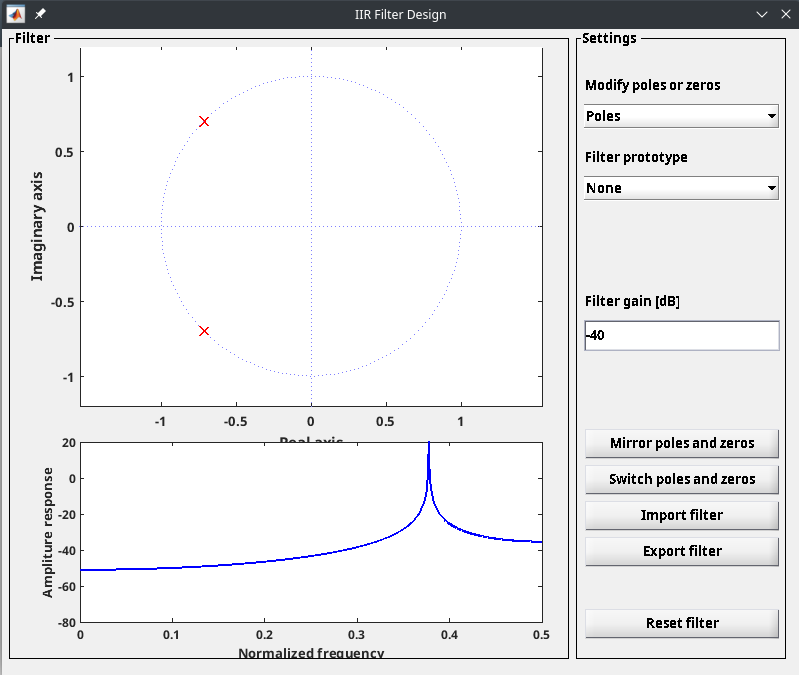
\includegraphics[scale=0.6]{./images/2ndorder-pole.png}
    \caption{Second order pole placed on the unit circle}
    \label{fig:my_label}
\end{figure}

Placing the poles on the unit circle will cause the system to be unstable.

Changing the $\omega$ from 0 to $\pi$ will only change the frequency where we attenuate. 
\subsection{Lab Task 6}
For task 6, the the same audio file used in previous tasks ('HQmusic.wav') was used. A sinusoid distortion with frequency $\frac{F_s}{4}$ was added in MATLAB. Figure 14 contains the power spectral density-plot of the distorted signal.
\begin{figure}[H]
    \hspace{-50pt}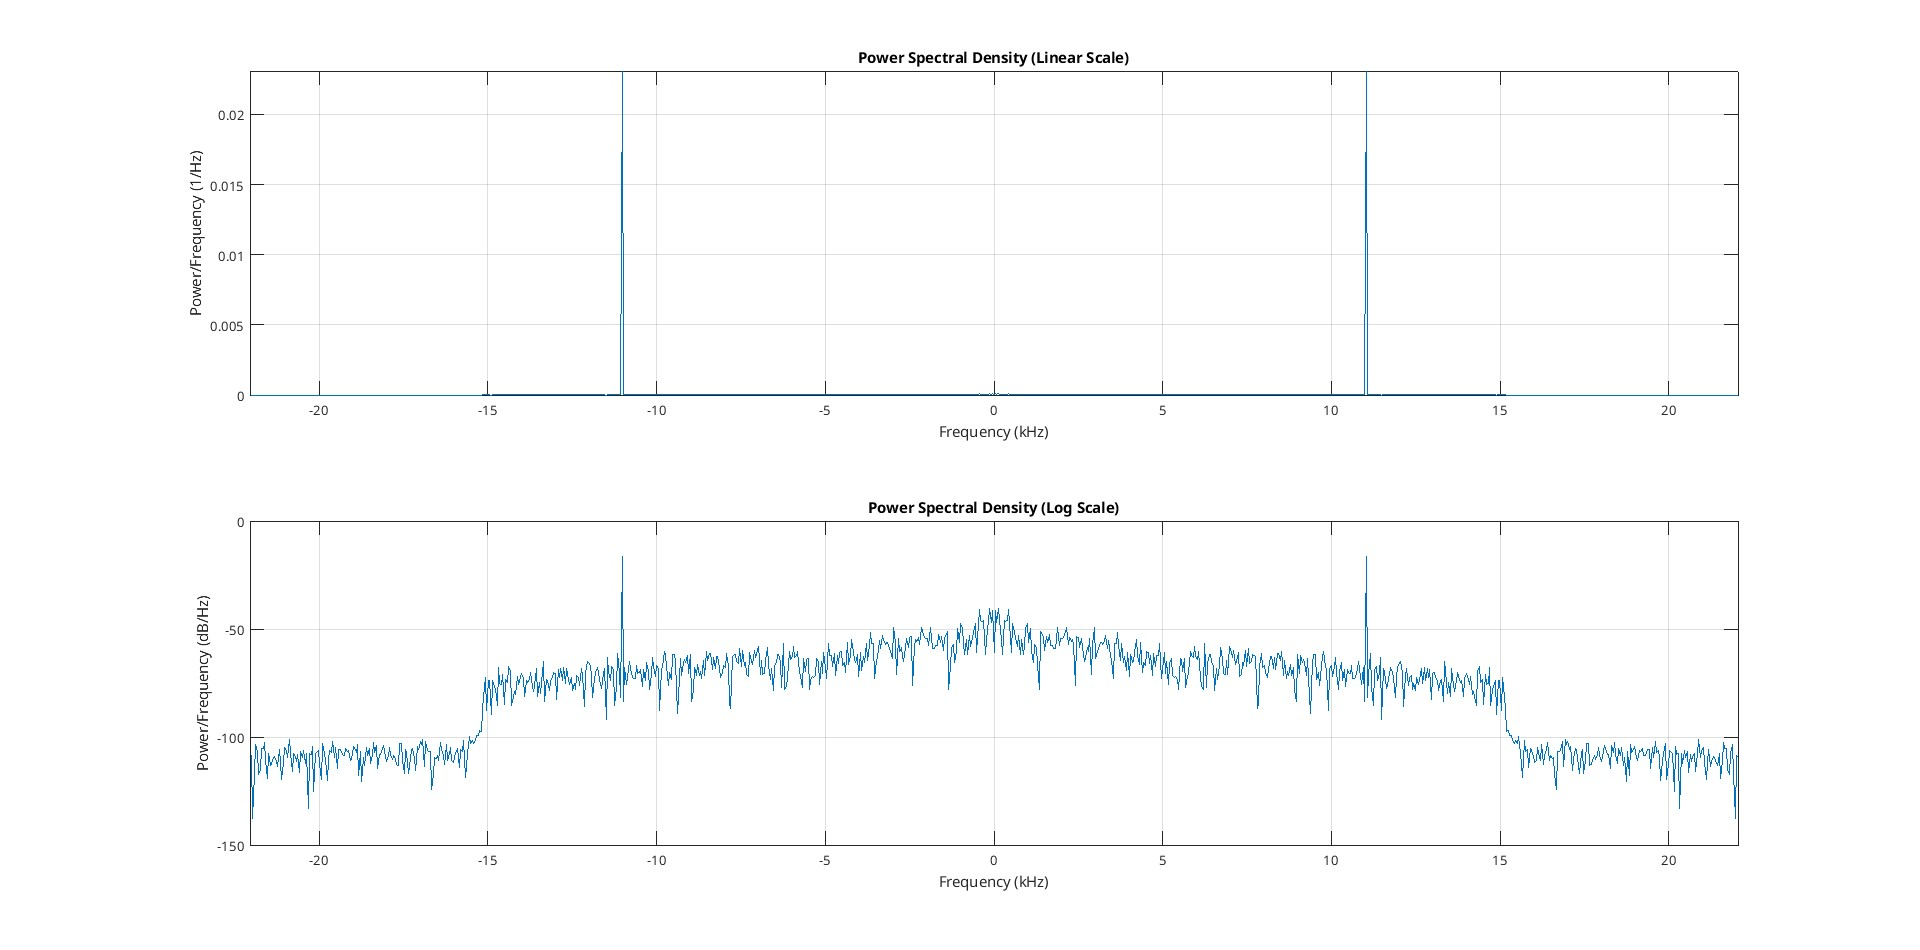
\includegraphics[scale=0.28]{./images/Task6-FFT.jpg}
    \caption{Frequency domain plot of the distorted signal created in task 6}
    \label{fig:my_label}
\end{figure}
Looking at the frequency domain signal, one can see clear spikes at $\sim$11 kHz, which corresponds to $\frac{F_s}{4}$ (where $F_s = 44100$kHz), as intended.
\subsection{Lab Task 7}
For task 7, a simple FIR filter with zeroes in \pm$\frac{\pi}{2}$ was constructed using the mkiir command in MATLAB. Since no poles were added, the signal quality decreased in a large band around the filtered frequencies ($\frac{F_s}{4}$). A frequency domain plot of the filtered signal can be found in figure 15.
\begin{figure}[H]
    \hspace{-45pt}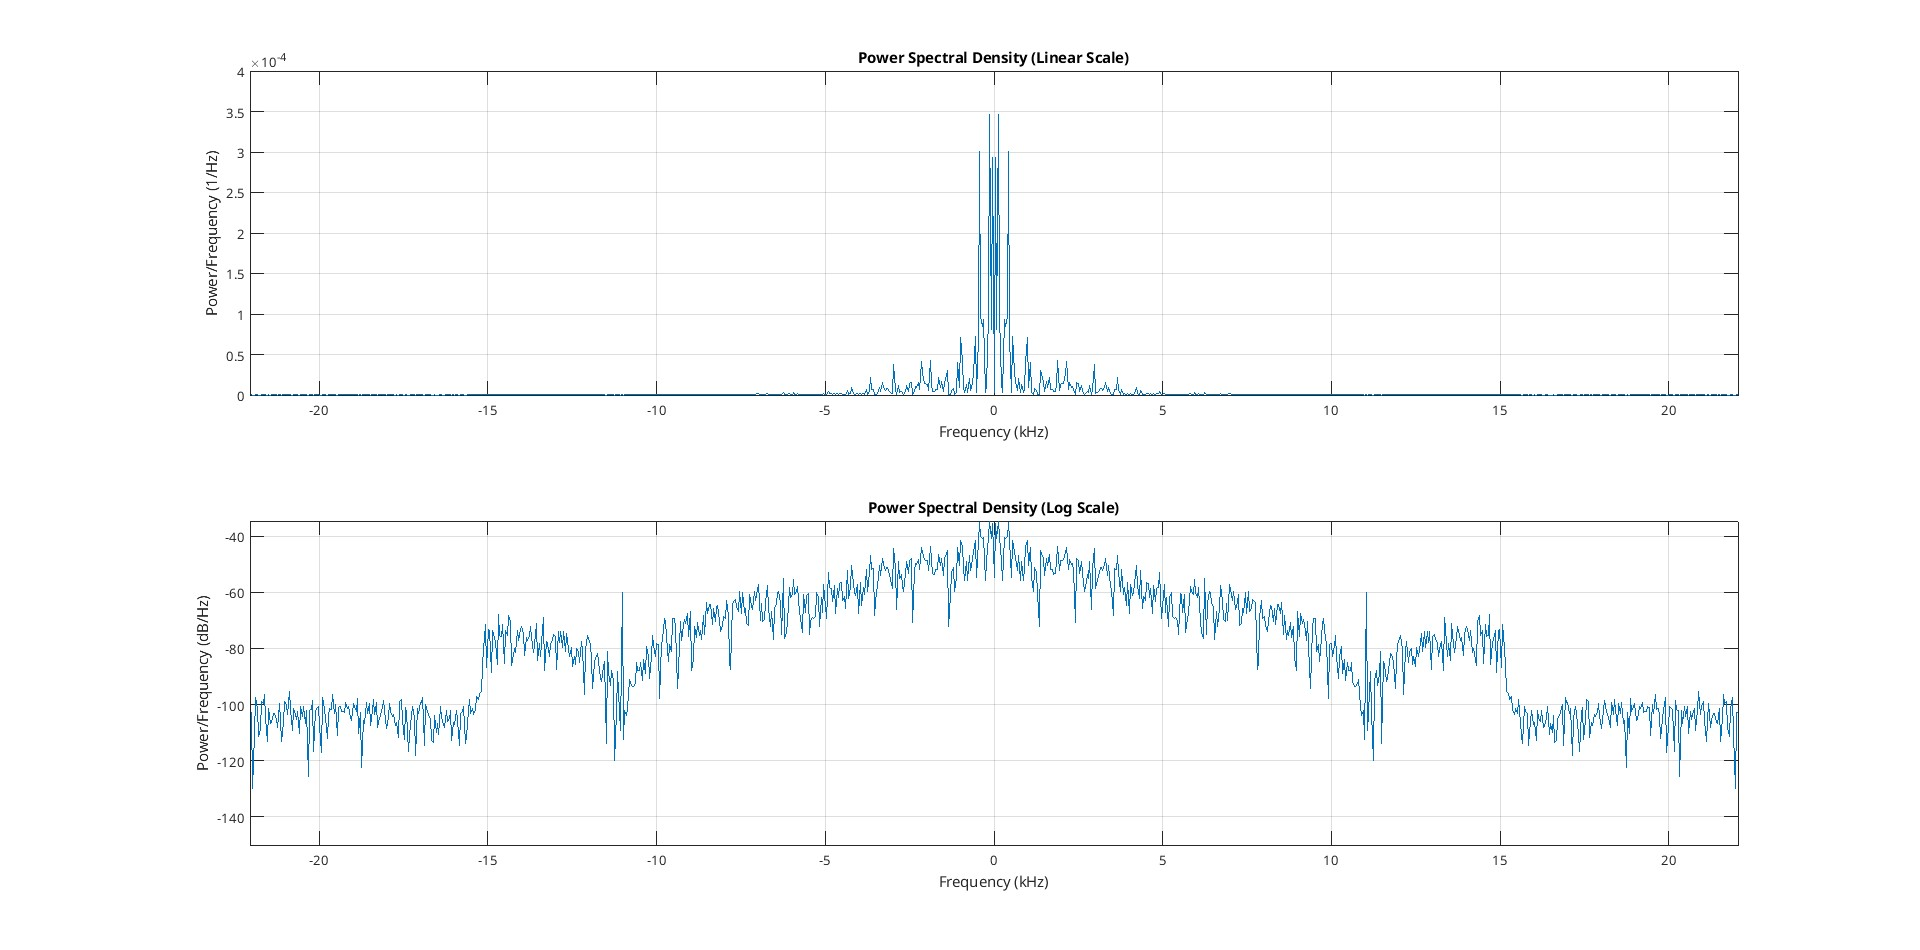
\includegraphics[scale=0.28]{./images/Task7-filtered.jpg}
    \caption{Signal plot after applying the FIR-filter constructed in task 7}
    \label{fig:my_label}
\end{figure}
\subsection{Lab Task 8}
For task 8, a FIR-filter was constructed. For this task a new (distorted) audio file was imported to MATLAB and plotted.
\begin{ffcode}
%% Task 8
[y2, f2] = audioread('MATLAB_FILES/distorted_music/lovesong.wav');
%soundsc(y2, f2)
Spectrum_PLOT(y2, f2)
\end{ffcode}
The plot can be seen in figure 16
\begin{figure}[H]
    \hspace{-40pt}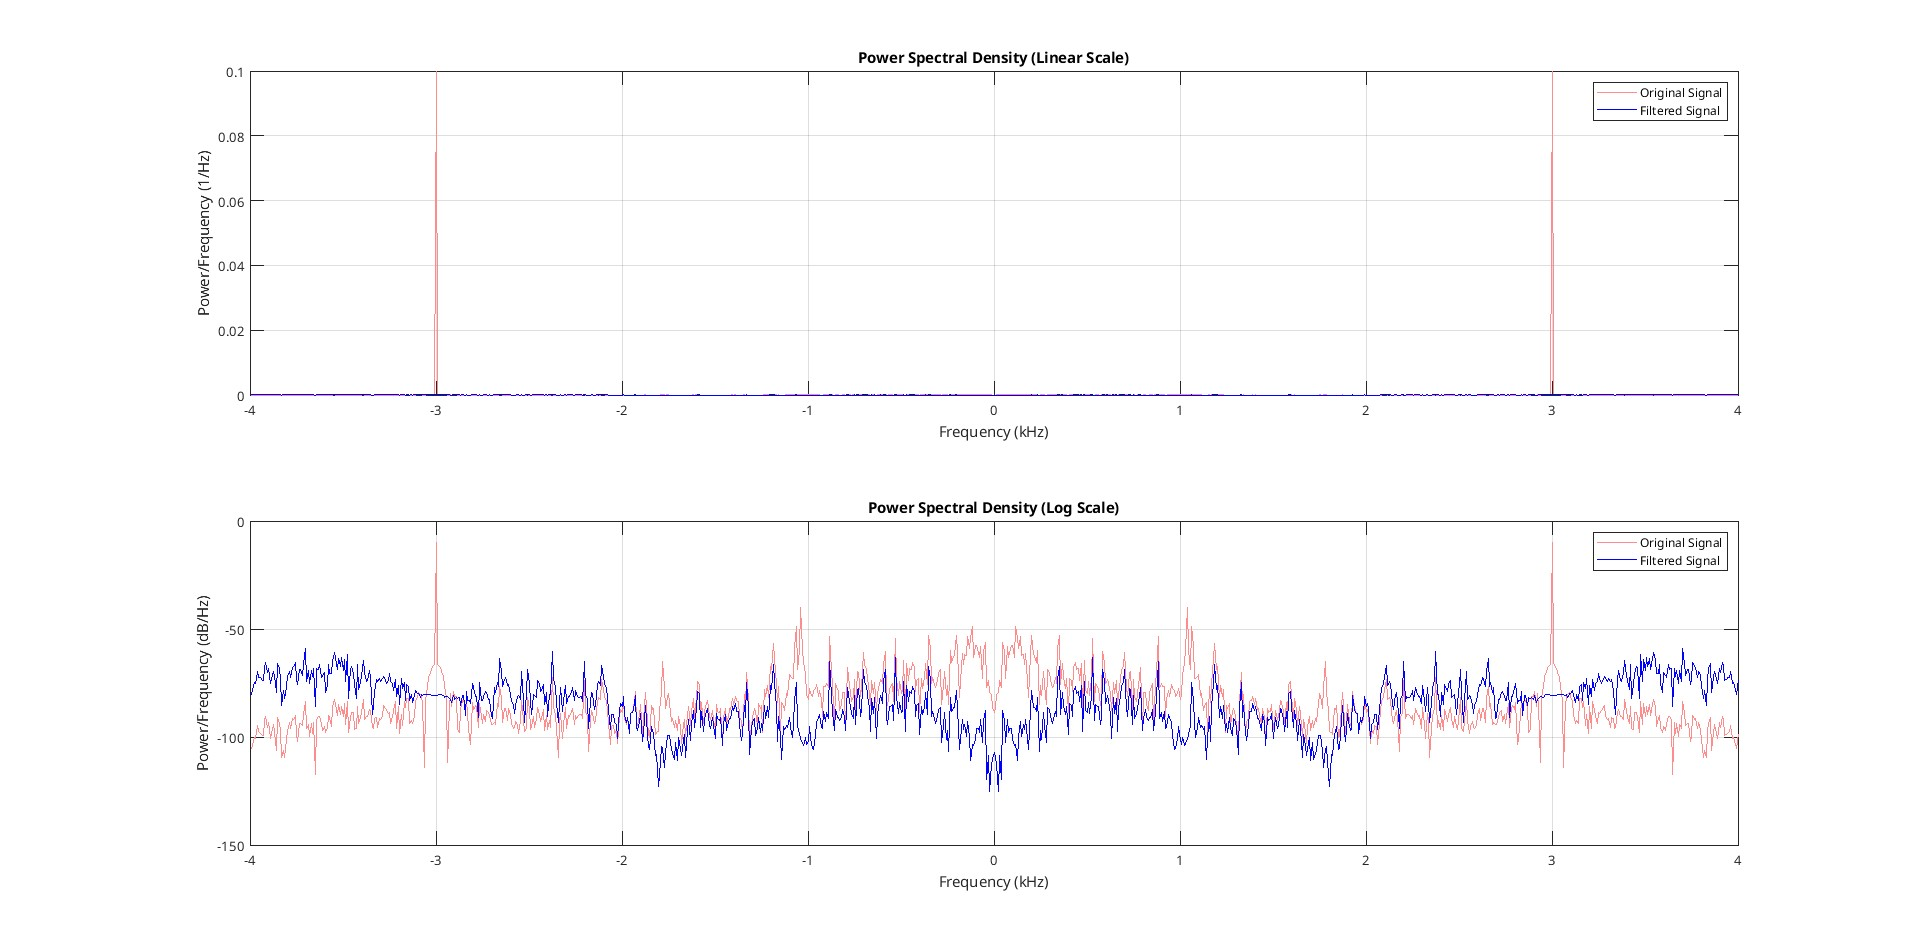
\includegraphics[scale=0.28]{./images/Task8-double-plot.jpg}
    \caption{Filtered music (blue) compared to non-filtered (red).}
    \label{fig:my_label}
\end{figure}

At first sight just studying the unfiltered signal, there's a distortion at $\pm$3kHz. After removing this, the high pitch noise in the signal could no longer be heard. Unfortunately there was some distortion at $\pm$1.78kHz, $\pm$1.04kHz and $\pm$0.12kHz. These distortions were removed in MATLAB:
\begin{ffcode}
%signal spikes at ±0.12kHz, ±1.04kHz, ±1.78kHz and ±3kHz
zeroes = 1.0e+3*[-0.12, 0.12, -1.04, 1.04, -1.78, 1.78, -3, 3] / f2;
zeroes = zeroes * (2 *  pi);
zeroes = exp(i * zeroes);
%as many poles as zeroes
poles = 0 * ones(1, length(zeroes));
b = poly(zeroes);
a = poly(poles);
y2_f = filter(b, a, y2);
Spectrum_PLOT(y2_f, f2);
soundsc(y2_f, f2)
Spectrum_DoublePLOT(y2, y2_f, f2)
\end{ffcode}
Removing these distortions  cleared the signal from most of the noise that was being heard. Even though there still a one tone noise in the background, the music quality was pretty good. You can also see the 2 high spikes in the unfiltered signal (red), and how they are absent from the filtered blue line. 

\subsection{Lab Task 9}
For task 9, the previous FIR-filter was replaced with an IIR-notch-filter with poles near the zeroes.
\begin{ffcode}
%% Task 9
[y2, f2] = audioread('MATLAB_FILES/distorted_music/lovesong.wav');
%soundsc(y2, f2)
Spectrum_PLOT(y2, f2)
%signal spikes at ±0.12kHz, ±1.04kHz, ±1.78kHz and ±3kHz
zeroes = 1.0e+3*[-0.12, 0.12, -1.04, 1.04, -1.78, 1.78, -3, 3] / f2;
zeroes = zeroes * (2 * pi);
zeroes = exp(i * zeroes);
%IIR notch, poles near zeroes
poles = 0.95 * zeroes;
b = poly(zeroes);
a = poly(poles);
y2_f = filter(b, a, y2);
Spectrum_PLOT(y2_f, f2);
soundsc(y2_f, f2)
Spectrum_DoublePLOT(y2, y2_f, f2)
\end{ffcode}
\begin{figure}[H]
    \hspace{-40pt}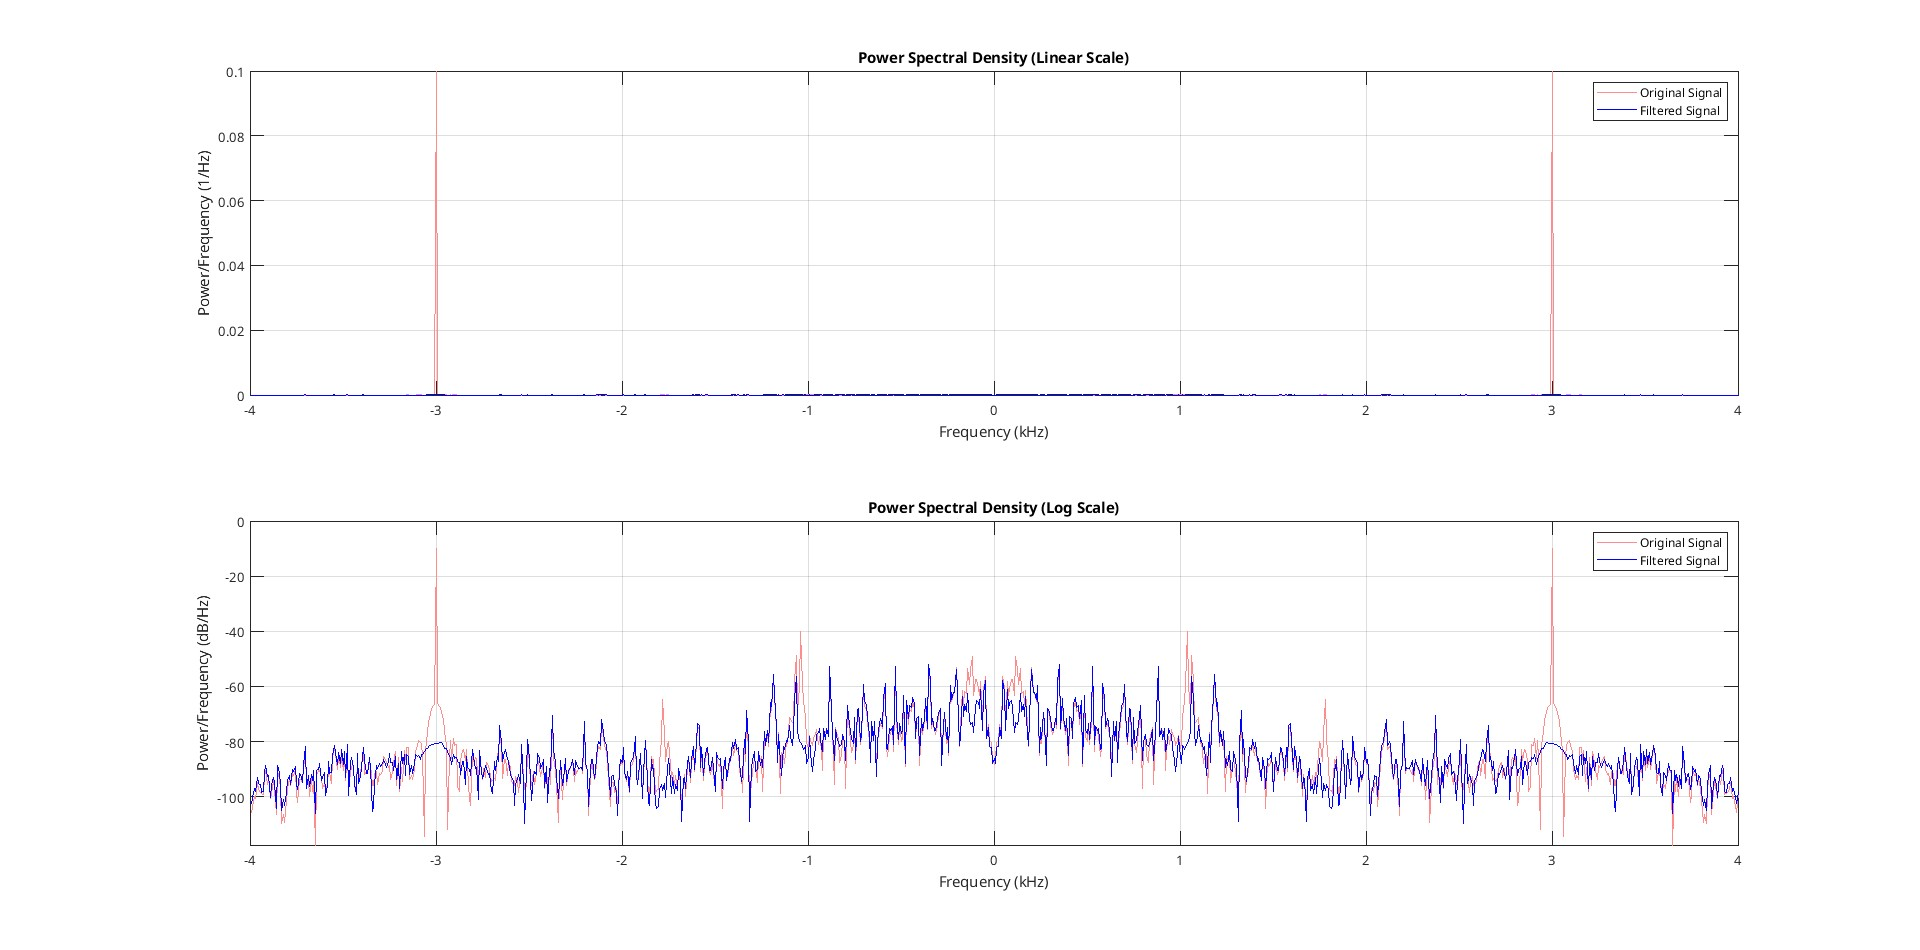
\includegraphics[scale=0.28]{./images/Task9-double-plot.jpg}
    \caption{Filtered music (blue) compared to non-filtered (red).}
    \label{fig:my_label}
\end{figure}


The music in Task 9 compared to Task 8 sounds fuller as well as louder. Listening to filtered music with more and more zeroes placed had the same effect as in task 8. 

\subsection{Lab Task 10}
For task 10, an echo corresponding to sound traveling 50m was added to a signal.
The delay in seconds was calculated as $t = \frac{distance}{time} = \frac{50}{340}$. This was then converted to samples by multiplying with the sample speed $D = t \cdot F_s$. A filter was constructed in MATLAB according to these calculations. The original and filtered signals were plotted and can be seen in figure 18.
\begin{ffcode}
%% Task 10
% Create echo
[y,f] = audioread('MATLAB_FILES/speech1.wav');
%soundsc(y, f)
delay = 50 / 340;
alpha = 0.8;
D = delay * f;
D = round(D);
b = [1, zeros(1, D), alpha];
poles = 0*ones(1, length(b));
a = poly(poles);
u = filter(b, a, y);
%create time vector
time = length(y) / f;
time = linspace(0, time, length(y));

%plot original signal (time domain)
subplot(2, 1, 1)
plot(time * f, y)
%plot echoed signal (time domain)
subplot(2, 1, 2)
plot(time * f, u)
%plot echoed signal (freq. domain)
Spectrum_PLOT(u, f)
%soundsc(u, f)
\end{ffcode}

\begin{figure}[H]
    \hspace{-40pt}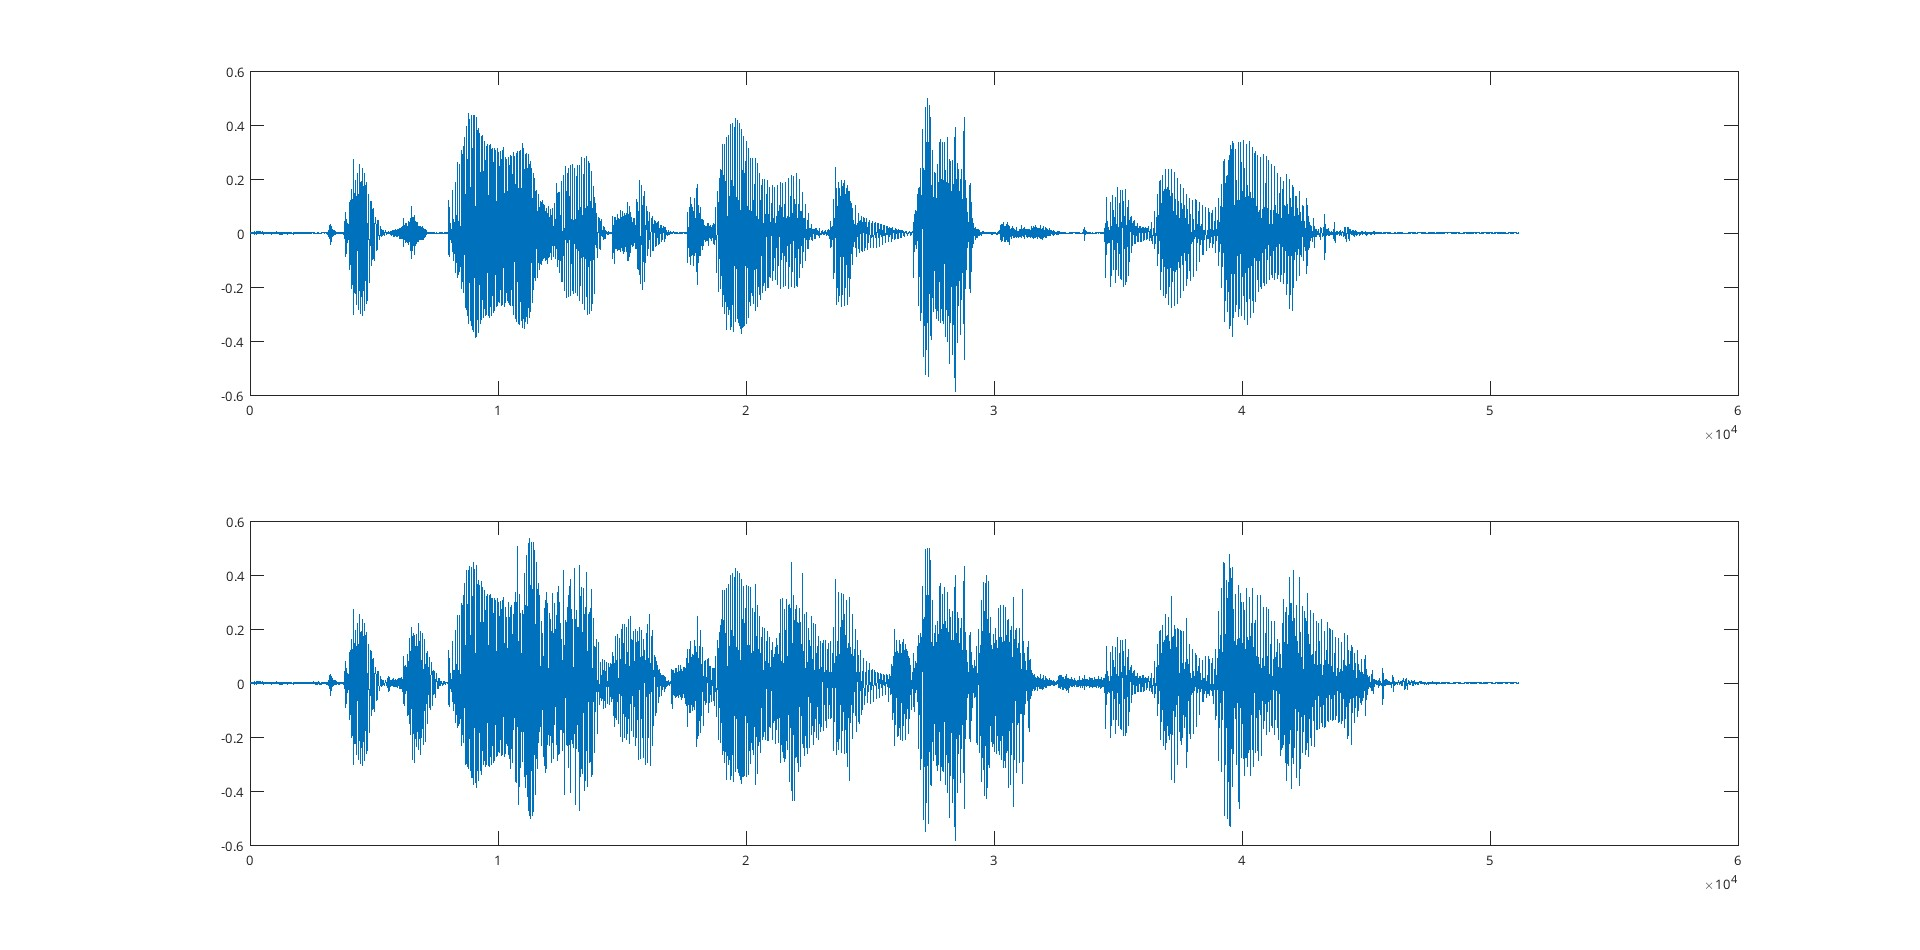
\includegraphics[scale=0.28]{./images/Task10-Echo.jpg}
    \caption{Original signal (top) and signal with applied echo (bottom).}
    \label{fig:my_label}
\end{figure}

 

Comparing the two signals in figure 18, one can see both signs of the echo and patterns of constructive interference. One clear instance of interference can be seen in the second part of the signals, where the amplitude of the filtered (echoed) signal is much larger than the original.

\subsection{Lab Task 11}
The echo was removed from the signal in task 11 by inverse filtering. A new filter was constructed with poles in the "echo-filters" zeroes to nullify the echo.  
\begin{ffcode}
%% Task 11
%create time vector
time = length(y) / f;
time = linspace(0, time, length(y));

% Remove echo by inverse filtering
a_new = [1, zeros(1, D), alpha];
b_new = 0*ones(1, length(a_new));
b_new = poly(b_new);
x = filter(b_new, a_new, u);
subplot(2, 2, 1, 'replace')
plot(time * f, y)
subplot(2, 2, 3)
plot(time * f, u)
subplot(2, 2, 2)
plot(time * f, x)
soundsc(x, f)
Spectrum_PLOT(x, f)
\end{ffcode}

\begin{figure}[H]
    \hspace{-40pt}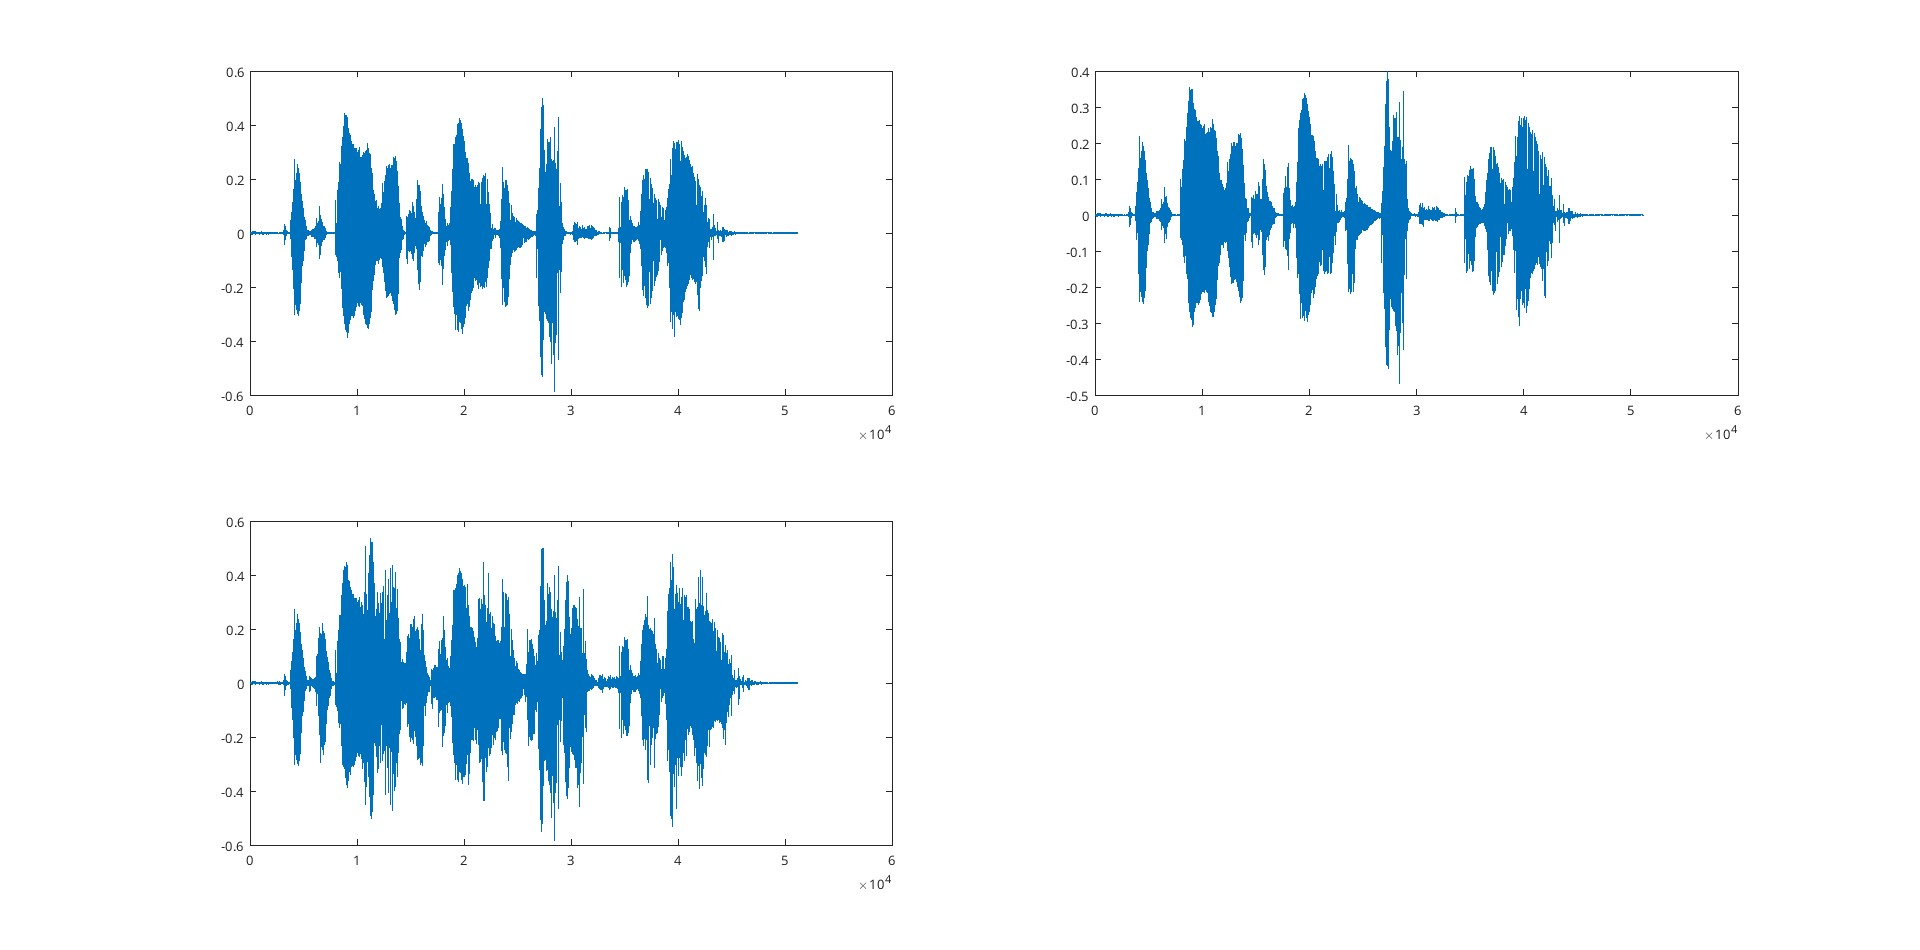
\includegraphics[scale=0.28]{./images/Task11.jpg}
    \caption{Original signal (top left), signal with applied echo (bottom) and signal with echo removed (top right.}
    \label{fig:my_label}
\end{figure}

We can see that inverse filtering brought back the original signal, however there are some minimal differences in amplitude. This is however, not discernible when listening to the signals side by side, meaning that it is likely a good filter for audio processing.

\end{document}